\newpage

\section{Time Constant of a Thermistor}
\label{s:time_constant}

\subsection{Parts List}

\begin{enumerate}[itemsep=-5pt]
\item CPX/CPB
\item USB Cable
\item Laptop
\end{enumerate}

\subsection{Learning Objectives}
\begin{enumerate}[itemsep=-5pt]
\item Learn the basic form of a first order system
\item Learn the basic solution of a first order system
\item Understand settling time and how that effects engineering
\item Applied Estimation of a First Order system
\end{enumerate}

\subsection{Getting Started}

The basic form of a first order system can be shown below.
\begin{equation}
\dot{T} = \sigma (T_f - T)
\end{equation}
where $T$ is our state variable and $\dot{T}$ is the derivative of our state. For this example let's assume that $T$ is temperature. In this case $T_f$ is an external temperature that is either higher or lower than current temperature causing the derivative of temperature to be non-zero. You can see in this case that once the temperature of the system is equal to the external forcing temperature, the derivative of the temperature of the system goes to zero. This implies that the system has reached equilibrium. The variable $\sigma$ has units of $Hz$ or $1/sec$. The inverse of $\sigma$ is $\tau$ the time constant.
\begin{equation}
\tau = \frac{1}{\sigma}
\end{equation}
The time constant of the system is related to how quickly the system responds to change or even how long it takes for the system to reach equilibrium. Reaching equilibrium quantitatively happens when the state has changed 98\%. In other words the state of the system is within 2\% of the equilibrium state. This is called the settling time $T_s$. The time constant is related to the settling time using the equation below.
\begin{equation}
\tau = \frac{T_s}{4}
\end{equation}
The only question now of course is what is the solution $T(t)$ or rather the temperature as a function of time. In this case, the solution to the above dynamics equation can be solved using \href{https://www.youtube.com/watch?v=VOv2HI3i7oo}{standard first order differential equation techniques} to obtain the solution below.
\begin{equation}\label{e:thermistor}
T(t) = (T_0-T_f)e^{-\sigma t} + T_f
\end{equation}
Looking at the equation now you can see some properties right away. When $t=0$, the first term reduces to $(T_0-T_f)$ which means the initial temperature is $T_0$ or the initial temperature. When $t\rightarrow\infty$, the first term drops to zero and thus the temperature is $T_f$ or final temperature.

\subsection{Temperature Change Ideas}

In this lab we’re going to get the time constant of the \href{https://en.wikipedia.org/wiki/Thermistor}{thermistor} on board the CPX. If you take data on the CPX and walk outside or place the thermistor directly into a fridge, the temperature change will not be immediate. Remember that the thermistor is a resistor that changes with temperature. The ADC on the CPX converts the voltage across the thermistor to temperature. \href{https://learn.adafruit.com/thermistor/circuitpython}{The Adafruit Learn system} does a bit of work to explain the conversion from voltage to temperature. My version of the code is also on my \href{https://github.com/cmontalvo251/Microcontrollers/blob/master/Circuit_Playground/CircuitPython/Temp/record_temperature_thermistor.py}{Github}.
\begin{figure}[H]
  \begin{center}
    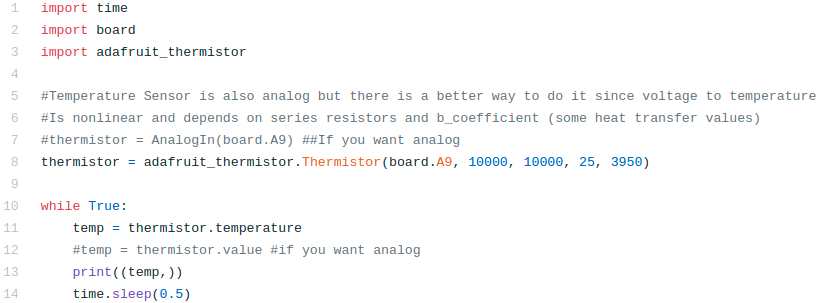
\includegraphics[width=\textwidth]{Figures/thermistor.png}
  \end{center}
\end{figure}
For this lab in order to estimate the time constant of a thermistor you need to change the temperature somehow.
\begin{enumerate}[itemsep=-5pt]
\item Start logging data and then place the CPX into the fridge
\item Put the CPX into the fridge and then pull the CPX out of the fridge and watch the temperature return to ambient
\item Walk outside on a hot (or cold) day and watch the CPX change temperature due to your A/C
\item Walk inside and watch the CPX get warmer (or colder) as your HVAC changes the CPX temperature.
\end{enumerate}

\subsection{Estimating Time Constant}
I did the first two examples and plotted both data sets in the same script as shown below. I opted to use method 1 (see chapter \ref{s:daq}) from the datalogging project and just have the data print to Serial and then unplug the CPX when I’m done taking data and copy and paste the data into a text file.
\begin{figure}[H]
  \begin{center}
    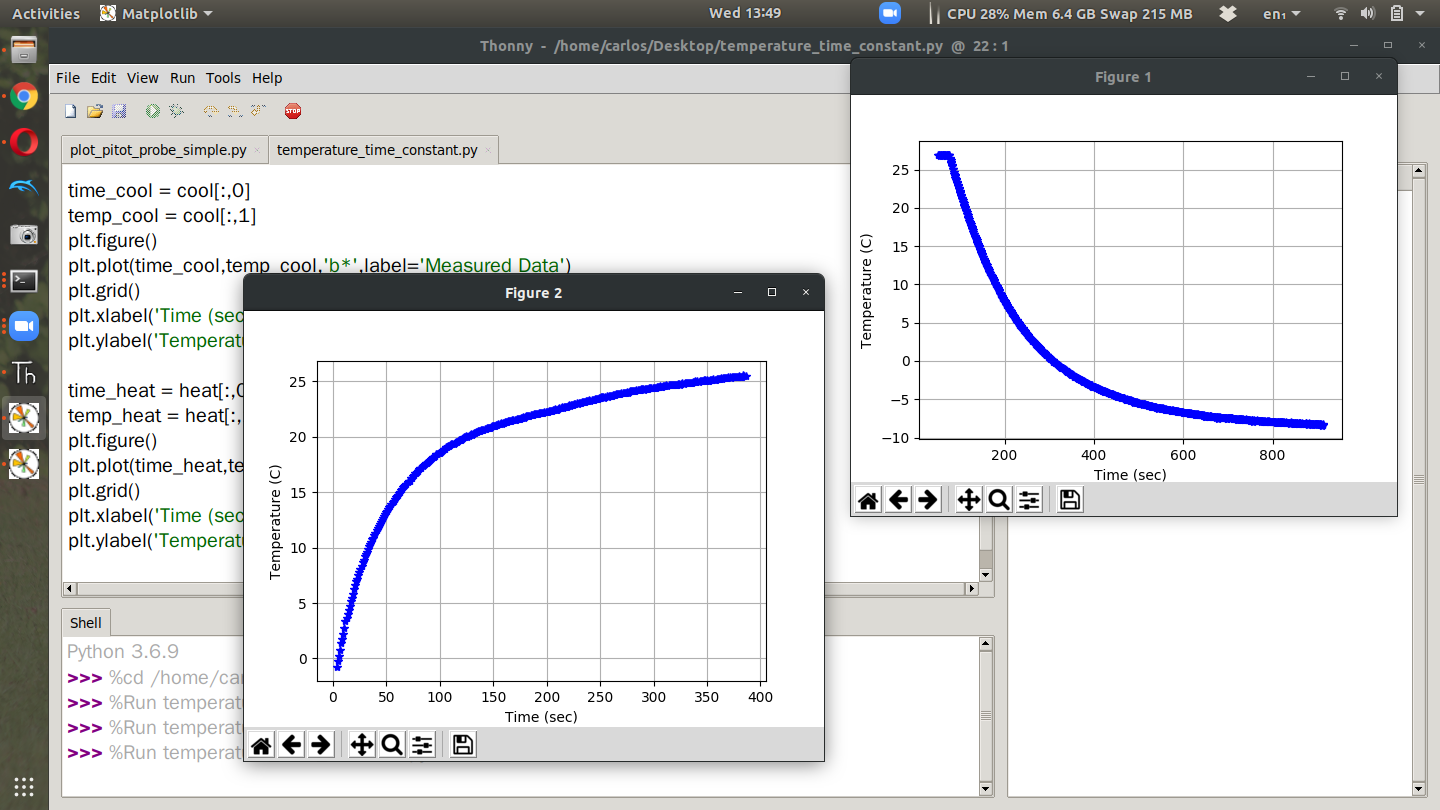
\includegraphics[width=\textwidth]{Figures/thermistor_plots.png}
  \end{center}
\end{figure}
At this point it’s possible to get the time constant by remember that the settling time (time it takes the temperature to settle out) is equal to 4 times the time constant ($\tau$) and thus the time constant is the settling time divided by 4. After computing the settling time for both data sets and overlaying the equations on the measured data I get these two plots.
\begin{figure}[H]
  \begin{center}
    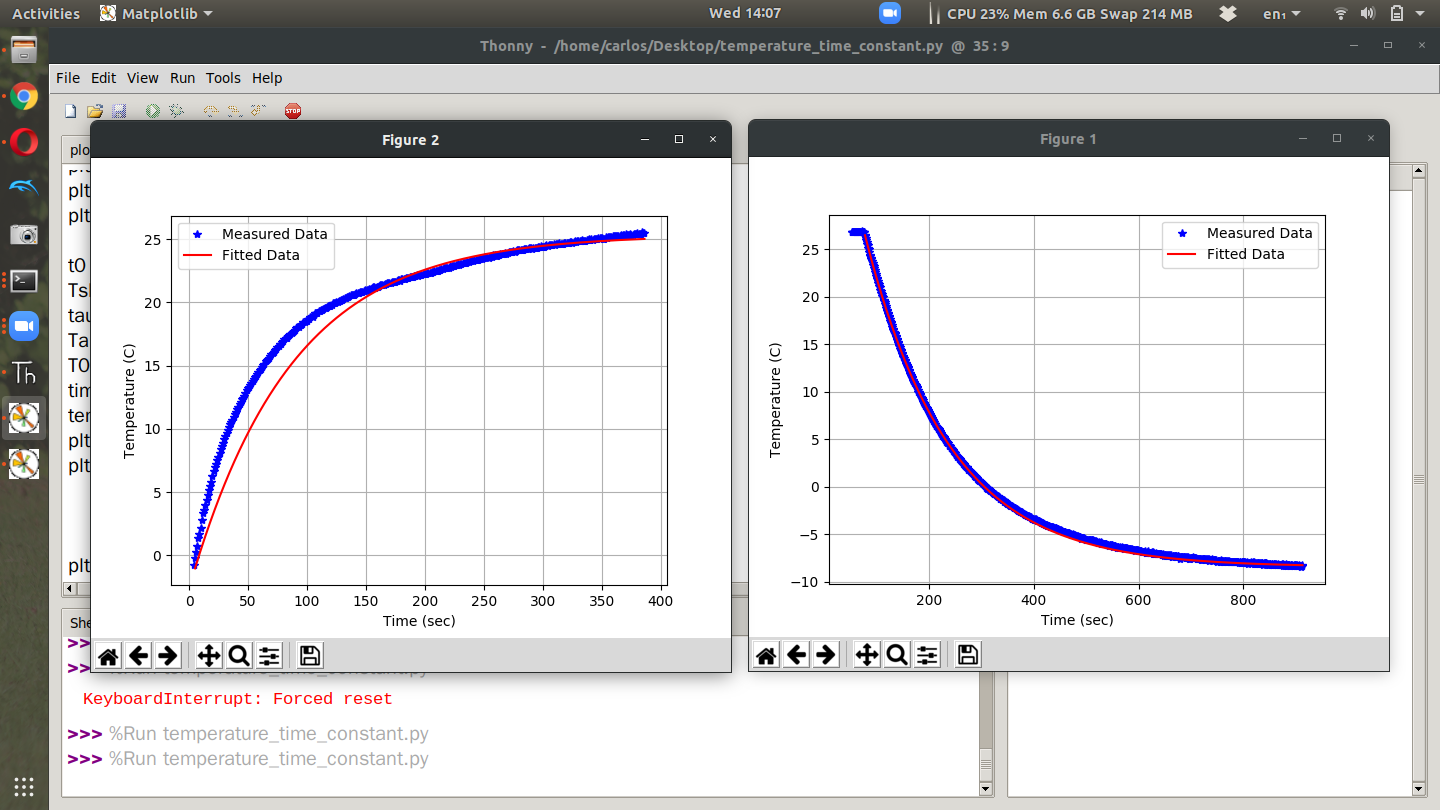
\includegraphics[width=\textwidth]{Figures/thermistor_plots2.png}
  \end{center}
\end{figure}
What was interesting was that the time constant for heating up was 62.5 seconds and for cooling down it was 155 seconds. The time to get cold was way slower than heating up. I’m not a heat transfer expert so I won’t comment as to why this happened. One other import note I’d like to mention is the cool down phase was much more accurate than the heat up phase. This is most likely because when I pulled the thermistor out of the fridge I touched it with my hands and then moved it to a table. There was also alot more airflow outside the fridge which would change the overall dynamics. Still, the fitted data matches up pretty well and I hope yours does too.

\subsection{Assignment}

For this assignment you are to change the ambient temperature of the CPX/CPB through heating or cooling and then record time and temperature while waiting for the CPX/CPB to return to ambient temperature. You are to then plot temperature as a function of time and then using the graph (not using a curve fit), estimate $T_0$, $T_f$,$\sigma$ and $\tau$. Finally, using equation \ref{e:thermistor}, plot the estimate of $T(t)$.

Once you've completed the project above, upload a PDF with all of the photos and text
below included. My recommendation is for you to create a Word document
and insert all the photos and text into the document. Then export the
Word document to a PDF. For videos I suggest uploading the videos to
Google Drive, turn on link sharing and include a link in your
PDF. Note that all code must be included in the appendix or you'll be
penalized 10\%. 


\begin{enumerate}[itemsep=-5pt]
\item Take a picture of you heating or cooling the CPX/CPB - 20\%
\item Plot your raw temperature data with time on the x-axis and temperature on the y-axis and overlay your fitted data on top of your measured data. Points will be given based on how well your fit is - 40\%
\item Include a table of your estimated parameters - 20\%
\end{enumerate}
